\begin{knitrout}
\definecolor{shadecolor}{rgb}{0.969, 0.969, 0.969}\color{fgcolor}\begin{kframe}
\begin{alltt}
\hlkwd{set.seed}\hlstd{(}\hlnum{2021}\hlstd{)}
\hlstd{n}  \hlkwb{<-} \hlnum{1000}
\hlstd{book}  \hlkwb{<-} \hlkwd{rnorm}\hlstd{(n)}
\hlstd{movie} \hlkwb{<-} \hlkwd{rnorm}\hlstd{(n)}
\hlkwd{plot}\hlstd{(book, movie)} \hlcom{# plot all the books and movies}
\hlkwd{abline}\hlstd{(}\hlkwd{lm}\hlstd{(movie}\hlopt{~}\hlstd{book))}
\end{alltt}
\end{kframe}\begin{figure}

{\centering 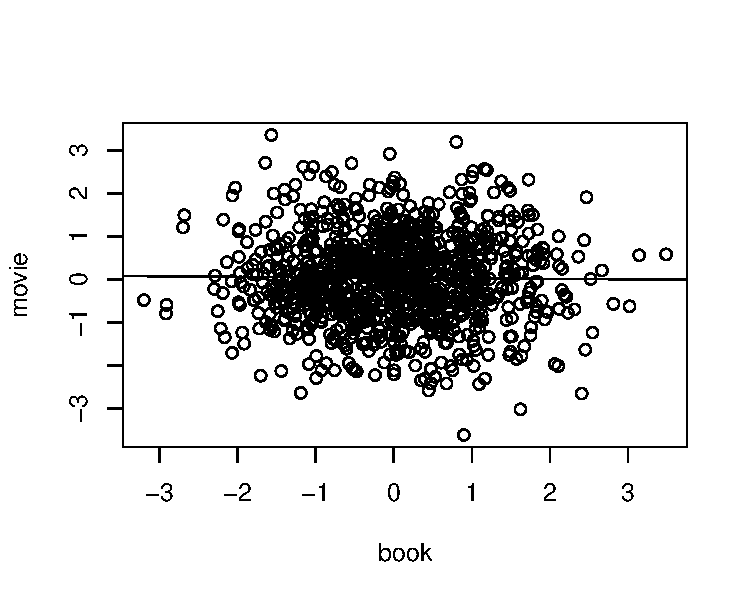
\includegraphics[width=\maxwidth]{figure/datacollect-Berkson-1} 

}

\caption[No linear association between goodness of movie and goodness of book]{No linear association between goodness of movie and goodness of book}\label{fig:datacollect-Berkson}
\end{figure}

\begin{kframe}\begin{alltt}
\hlkwd{cor}\hlstd{(book, movie)}
\end{alltt}
\begin{verbatim}
[1] -0.01178458
\end{verbatim}
\end{kframe}
\end{knitrout}

\begin{knitrout}
\definecolor{shadecolor}{rgb}{0.969, 0.969, 0.969}\color{fgcolor}\begin{kframe}
\begin{alltt}
\hlstd{good.b} \hlkwb{<-} \hlstd{book} \hlopt{>} \hlkwd{quantile}\hlstd{(book,} \hlnum{0.9}\hlstd{)}
\hlstd{good.m} \hlkwb{<-} \hlstd{movie} \hlopt{>} \hlkwd{quantile}\hlstd{(movie,} \hlnum{0.9}\hlstd{)}
\hlstd{good}  \hlkwb{<-} \hlstd{good.b} \hlopt{|} \hlstd{good.m}
\hlkwd{plot}\hlstd{(book[good], movie[good])} \hlcom{# plot only the good books or good movies}
\hlkwd{abline}\hlstd{(}\hlkwd{lm}\hlstd{(movie[good]}\hlopt{~}\hlstd{book[good]))}
\end{alltt}
\end{kframe}\begin{figure}

{\centering 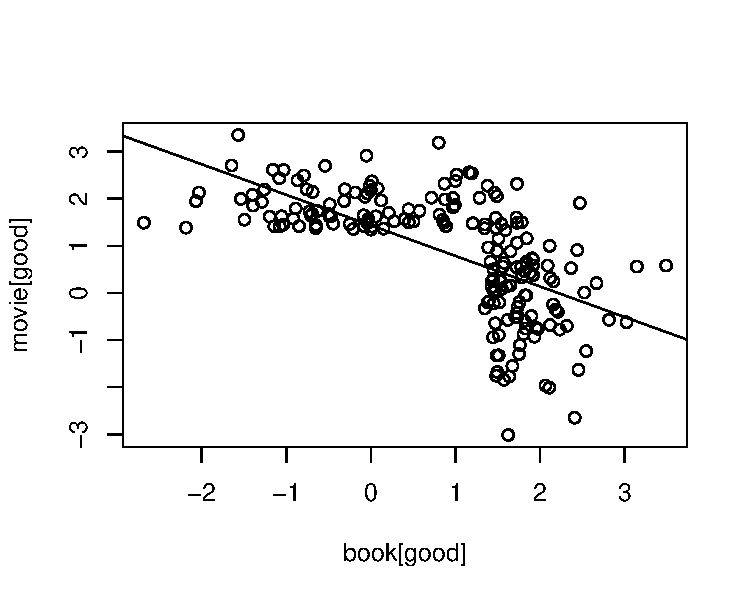
\includegraphics[width=\maxwidth]{figure/datacollect-Berkson2-1} 

}

\caption[Negative linear association for top 10 percent books and/or movie]{Negative linear association for top 10 percent books and/or movie}\label{fig:datacollect-Berkson2}
\end{figure}

\begin{kframe}\begin{alltt}
\hlkwd{cor}\hlstd{(book[good], movie[good])}
\end{alltt}
\begin{verbatim}
[1] -0.6394144
\end{verbatim}
\end{kframe}
\end{knitrout}
